% Use only LaTeX2e, calling the article.cls class and 12-point type.
\documentclass[12pt]{article}

% Users of the {thebibliography} environment or BibTeX should use the
% scicite.sty package, downloadable from *Science* at
% www.sciencemag.org/about/authors/prep/TeX_help/ .
% This package should properly format in-text
% reference calls and reference-list numbers.

\usepackage{scicite}

% Use times if you have the font installed; otherwise, comment out the
% following line.

\usepackage{times}
\usepackage[utf8x]{inputenc}
\usepackage{scicite}
\usepackage{graphicx}
\usepackage{amsmath}
\usepackage{hyperref}
\usepackage{makeidx}
\usepackage[italian]{babel}
\usepackage[colorinlistoftodos]{todonotes}


\usepackage{times}
\usepackage{listings}


\lstset{frame=tb,
  language=Xml,
  aboveskip=3mm,
  belowskip=3mm,
  showstringspaces=false,
  columns=flexible,
  basicstyle={\small\ttfamily},
  numbers=none,
  breaklines=true,
  breakatwhitespace=true,
  tabsize=3
}

% The preamble here sets up a lot of new/revised commands and
% environments.  It's annoying, but please do *not* try to strip these
% out into a separate .sty file (which could lead to the loss of some
% information when we convert the file to other formats).  Instead, keep
% them in the preamble of your main LaTeX source file.


% The following parameters seem to provide a reasonable page setup.

\topmargin 0.0cm
\oddsidemargin 0.2cm
\textwidth 16cm 
\textheight 21cm
\footskip 1.0cm


%The next command sets up an environment for the abstract to your paper.

\newenvironment{sciabstract}{%
\begin{quote} \bf}
{\end{quote}}


% If your reference list includes text notes as well as references,
% include the following line; otherwise, comment it out.

\renewcommand\refname{References and Notes}

% The following lines set up an environment for the last note in the
% reference list, which commonly includes acknowledgments of funding,
% help, etc.  It's intended for users of BibTeX or the {thebibliography}
% environment.  Users who are hand-coding their references at the end
% using a list environment such as {enumerate} can simply add another
% item at the end, and it will be numbered automatically.

\newcounter{lastnote}
\newenvironment{scilastnote}{%
\setcounter{lastnote}{\value{enumiv}}%
\addtocounter{lastnote}{+1}%
\begin{list}%
{\arabic{lastnote}.}
{\setlength{\leftmargin}{.22in}}
{\setlength{\labelsep}{.5em}}}
{\end{list}}

\title{Elaborazione del linguaggio naturale} 

\author{Simone Scala,$^{1}$ Bartolomeo Lombardi$^{2}$\\
    \\
    \textbf{Corso di laurea magistrale in Informatica} \\
    \textbf{Università di Bologna}
    \\\\
    \normalsize{$^{1}$simone.scala3@studio.unibo.it,}\\
    \normalsize{$^{2}$bartolomeo.lombardi@studio.unibo.it}\\
}

% Include the date command, but leave its argument blank.

\date{01 Febbraio 2017}

%%%%%%%%%%%%%%%%% END OF PREAMBLE %%%%%%%%%%%%%%%%

\begin{document} 

% Double-space the manuscript.

\baselineskip 24pt

\maketitle 

\begin{sciabstract}
  Il linguaggio è un fenomeno complesso e raramente viene inteso come sia prodotto e percepito. Un primo approccio intuitivo può indurre a pensare che il linguaggio sia costituito da parole e ogni parola sia costituita da fonemi, ma questo è certamente non vero. Il linguaggio è un processo dinamico, ove le varie parti sono raramente distinguibili. In questo progetto,  mediante \textit{CMUSphinx}, toolkit open source utilizzato per creare e allenare modelli acustici, si è tentato di sviluppare un riconoscitore vocale che riuscisse ad interpretare una serie di comandi. ........(da completare)..........
\end{sciabstract}

\newpage
\tableofcontents
\newpage

\section{Introduzione}
    In questa sezione introduttiva cercheremo di descrivere alcuni concetti che si collocano alla base del lavoro svolto.
    
    \begin{figure}
            \centering
            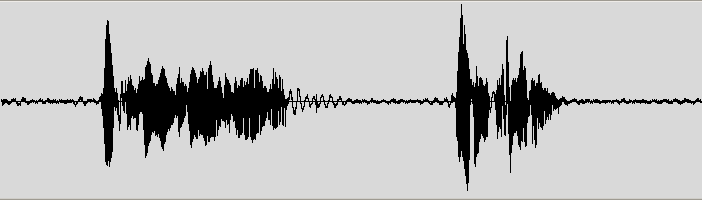
\includegraphics[scale=0.5]{waveform}
            \caption{Struttura di un waveform}
            \label{fig:first}
     \end{figure}

    \subsection{Struttura del linguaggio}
    
    Il linguaggio è un flusso d'audio continuo (fig:\ref{fig:first}) in cui gli stati piuttosto stabili si mescolano con gli stati evolutosi in modo dinamico. In questa sequenza di stati possono essere definite classi di suoni (o \textbf{foni}) più o meno equivalenti. Le proprietà acustiche di un flusso d'audio (\textbf{waveform}) corrispondente ad un fono sono spesso soggette al fenomeno della \textbf{coarticolazione}, per il quale ogni fono subisce l'influenza del contesto nel quale è articolato, vale a dire dei foni che lo precedono o lo seguono.
    L'effetto della coarticolazione può essere catturato dai \textbf{triphones}, che accorpano un singolo fono con quello immediatamente successivo e precedente. Per esempio, il fono \textit{c}  nella parola \textit{bocca} viene accorpato con il fono destro \textit{a} e con il fono sinistro \textit{c} che suona in maniera diversa rispetto allo stesso fono \textit{c} con fono destro \textit{e} e fono sinistro \textit{c} nella parola \textit{bocce}.
    L'operazione riguardante la costruzione dei triphones può risultare pesante dal punto di vista computazionale, risulta utile in tal senso individuare le parti di un triphones, anziché i triphones nel loro complesso. 
    Vengono quindi definiti detector distinti di suoni più brevi, che possano rappresentare l'intera varietà di rilevazioni acustiche. 
    Tali detector vengono chiamati \textbf{senones}.\\
    \textbf{N.B.}: un contesto potrebbe non dipendere semplicemente dal fono successivo e precedente. Piuttosto può dipendere da una funzione molto più complessa definita da un albero di decisione, o in altro modo.\\
    Un altro elemento chiave del linguaggio è rappresentato dalle \textbf{parole}, in quanto restringono in maniera significativa la dimensione dell'insieme derivante dalla combinazione dei foni. Ad esempio, se ci sono $40$ foni e una parola in media è composta da $7$ foni, possiamo avere al più $40^7$ parole, anzichè $40^{40}$.  
        
    \subsection{Processo di riconoscimento}    
    
    In generale, il processo di riconoscimento di un linguaggio consiste nel effettuare un attenta analisi del flusso d'audio registrato, ove quest'ultimo viene manipolato come segue:
    \begin{enumerate}
    \item viene estratto il \textit{waveform} dal flusso e viene frazionato in espressioni riconducibili alle parti stabili del grafico (silenzi)
    \item si prova poi a riconoscere cosa è stato detto in ogni espressione:
    \begin{itemize}
         
        \item calcolando tutte le possibili combinazioni tra le parole
        \item ricercando le corrispondenze audio-parola
        \item scegliendo la corrispondenza migliore dal punto di vista probabilistico 
    \end{itemize}
       % il \textit{waveform} viene frazionato in espressioni riconducibili alla parte stabile del grafico (silenzi), poi si prova a riconoscere cosa è stato detto in ogni espressione. A tal fine è necessario prendere in considerazione le combinazioni tra le parole, e provare a far corrispondere quest'ultime con l'audio scegliendo la corrispondenza migliore.%
    \end{enumerate}
    
    Riguardo il processo che definisce la corrispondenza audio-parola, ci sono ulteriori concetti che devono essere chiariti; il primo tra questi è il concetto di \textbf{features vector}: vettore costituito da una serie di numeri calcolati su un singolo frame, ottenuto dividendo il \textit{wavefrom} in intervalli regolari.
    Il metodo utilizzato per la generazione di tali numeri è oggetto di ricerca attiva (basata su regole), che nel caso più semplice, è derivata dallo spettro di frequenza. Il secondo, è quello di \textbf{modello}, nel quale vengono definiti oggetti matematici in grado di raccogliere gli attributi comuni della parola detta. Ricavando, quindi, il \textit{features vector} più probabile. Il modello del linguaggio è chiamato \textbf{Hidden Markov Model} (HMM), ove il processo di modellazione è descritto come una sequenza di stati, i quali si evolvono con una certa probabilità. Lo scopo di questo modello è quello di descrivere qualsiasi processo sequenziale come un linguaggio.    
    
    \subsection {Definizione dei modelli}
    A seconda della struttura del linguaggio, devono essere definiti tre oggetti affinché il sistema possa sviluppare il riconoscitore vocale:
        \begin{enumerate}
            \item Modello acustico: contiene le proprietà acustiche per ogni \textit{senone}.
            \item Dizionario della fonetica: mappa le parole con i foni; può essere definito mediante funzioni complesse, apprese con algoritmi di machine learning.
            \item Modello linguistico: usato per ottimizzare la ricerca della parola; definisce, quindi, quale parola potrebbe seguire quella precedentemente riconosciuta, riducendo così, la dimensione dell'insieme derivante dalla corrispondenza audio-parola, eliminando quelle parole che non hanno probabilità di comparire. Il modello linguistico più usato è \textbf{n-gram lenguage models} che contiene informazioni di tipo statistico riguardo la **successione delle parole.
        \end{enumerate}

    La combinazione di quest'ultimi permette al sistema \textbf{CMUSphinx} di elaborare il riconoscitore, 

\newpage
\section{Tecnologie utilizzate}
    In questo paragrafo verranno brevemente descritte le principali tecnologie utilizzate durante la realizzazione del progetto.
    
    \begin{enumerate}
    
        \item \textbf{CMUSphinx}: toolkit open source utilizzato per lo sviluppo di riconoscitori vocali. Contiene una serie di pacchetti utili allo sviluppo, quelli da noi utilizzati sono i seguenti:
         \begin{itemize}         
            \item \textbf{Pocketsphinx}: libreria utilizzata per interfacciarsi con il riconoscitore implementato (scritta in C).
            \item \textbf{Sphinxbase}: libreria di supporto richiesta per \textit{Pocketsphinx}. 
            \item \textbf{Sphinxtrain}: tool utilizzato nella fase di apprendimento del modello acustico.
        \end{itemize}
        
        \item \textbf{SRI Language Modeling (Srlim)}: toolkit che offre strumenti per costruire e applicare modelli linguistici statistici (LMs). Il toolkit viene rilasciato con licenza open source, infatti può essere scaricato e usato in maniera del tutto gratuita.
        
        \item \textbf{Sequence-to-Sequence G2P}: toolkit, anch'esso open source, utilizzato per la conversione parola-fonema; opera attraverso reti neurali ricorrenti (RNN) con architettura \textbf{LSTM} (long short-term memory). L'implementazione, è basata su \textit{TensorFlow}, libreria software open source per l'apprendimento automatico in diversi tipi di compiti percettivi e di comprensione del linguaggio, la quale consente un'efficiente fase di apprendimento.
        
        \item \textbf{Android}: sistema operativo per dispositivi mobili, adoperato durante lo sviluppo dell'applicativo, il quale, mediante l'interfacciamento con la libreria \textit{Pocketsphinx}, ci ha permesso di testare il riconoscitore.
    
    \end{enumerate}
  
\newpage
\section{Preparazione dei dati}
    Il sistema apprende i parametri che definiscono il modello acustico attraverso una serie di campioni audio, che vengono mantenuti in un database detto \textit{training database}. Tale database conterrà quindi le informazioni, le cui derivazioni statistiche, permetteranno il funzionamento del modello acustico.\\
    La prima fase è consista quindi nel raccogliere tali campioni; in tal senso abbiamo registrato $30$ voci, $15$ di sesso maschile e $15$ di sesso femminile, ove ogni speaker ha pronunciato gli undici comandi da noi stilati. In conclusione il nostro database di training conterrà $330$ registrazioni ($30$ voci $*$ $11$ comandi). Fondamentale in questa fase è stato assicurarsi che tutte le registrazioni fossero state registrate ad una frequenza di $16 Hz$ in mono stereo, così come suggerito dalla documentazione fornita da \textit{CMUSphinx}.\\       
    Ogni campione audio contenuto nel database deve essere poi etichettato, facendo  corrispondere quest'ultimo con la trascrizione della sequenza di parole contenuta nell'unità audio.  
    Tale etichettatura viene effettuata attraverso un file detto \textit{transcript file}, nel quale le sequenze di parole sono scritte esattamente nello stesso ordine con cui compaiono nell'audio, seguite da un tag $<s>$ che associa tale sequenza (frase) con la corrispettiva registrazione.
    Riportiamo a titolo esemplificativo una parte di tale file, così come descritto nel nostro modello, ove per ogni comando (valore del tag $<s>$) viene fatto corrispondere il file $wav$ contenente la registrazione dello speaker $anna$: 
    \newpage
    \begin{lstlisting}
    <s> apri impostazioni </s> (/anna/file_1)
    <s> apri contatti </s> (/anna/file_2)
    <s> dove mi trovo </s> (/anna/file_3)
    <s> apri calcolatrice </s> (/anna/file_4)
    <s> apri calendario </s> (/anna/file_5)
    <s> componi numero </s> (/anna/file_6)
    <s> chiama tre tre uno sei tre cinque sei sei zero quattro </s> (/anna/file_7)
    <s> chiama tre tre tre due zero due sette nove otto uno </s> (/anna/file_8)
    <s> chiama tre tre tre uno zero cinque zero due otto nove </s> (/anna/file_9)
    <s> chiama zero due sette otto quattro due quattro otto otto tre </s> (/anna/file_10)    
    \end{lstlisting}
    
    Il sistema poi necessita di un dizionario, che stabilisce una corrispondenza tra la parola e le unità sonore (foni) che la compongono, in modo tale da poter derivare la sequenza di foni associati ad un segnale.  
    
    
    \subsection{Costruzione del dizionario}
    
    La maggior parte delle parole, presenti nel \textit{transcript file} soprascritto, non erano contenute nel dizionario d'italiano scaricabile da \textit{CMUSphinx}, ragion per cui si è ricercato un tool, che fosse in grado di mappare le parole mancanti con la sequenza fonetica corrispondente.
    A tale scopo è stato utilizzato il toolkit \textit{G2P-seq2seq} che consente, partendo da un dizionario e un modello esistente,  di apprendere regole per la generazioni di sequenze di foni su parole "non viste" (non presenti nel dizionario di partenza).  
    Dopo aver installato tale toolkit, per avviare il training è stato sufficiente lanciare il comando: 
    \begin{lstlisting}
      g2p-seq2seq --train train-dictionary.dic --model model-folder-path
    \end{lstlisting}
    ove i parametri \textit{train-dictionary.dic} e \textit{model-folder-path} stanno ad indicare i dati su cui effettuare il training.
    Dopodichè, per generale la pronuncia, è stato lanciato il comando:
    \newpage
    \begin{lstlisting}
    g2p-seq2seq --interactive --model model_folder_path
        
        > impostazioni
        i m p o s t a ts ts j o1 n i
    \end{lstlisting}
    ove è stato possibile generare la la sequenza di foni, data la parola in input (nel esempio: "impostazioni")
    Dopo aver iterato tale procedimento, per ogni parola presente nel \textit{transcript file}, abbiamo finalmente ottenuto il nostro dizionario, che riportiamo a scopo esemplificativo.
    \begin{lstlisting}
    a a1
    a' a1
    apri a1 p r i
    calcolatrice k a1 l k o l a1 t r i tSS e
    calendario k a l e1 n d a1 r j o
    cancella k a n tSS EE l l a
    chiama k j a1 m a
    cinque tSS i1 ng k w e
    componi k o1 m p o n i
    contatti k o n t a1 t t i
    dove d o1 v e
    due d u1 e
    impostazioni i m p OO s t a ts ts j o1 n i
    mi m i1
    nove n OO v e
    numero n u1 m e r o
    otto OO t t o
    quattro k w a1 t t r o
    sei s EE i
    sette s EE t t e
    tre t r EE
    trovo t r OO v o
    uno u1 n o
    zero ts e1 r o 
    \end{lstlisting}
    
    \subsection{Costruzione del modello linguistico}
    
    
    * comandi utilizzati/ inizializzati
    * costruzione del dataset ( registrazioni e roba varia)
    * come abbiamo costruito il modello linguistico ? 
    * come abbiamo creato il dizionario ? 
    * come abbiamo configurato i parametri per il training.

\section{Fase di apprendimento}
    \subsection{Modello specializzato}
    * comandi per il training (come istruzioni)
    \subsection{Modello di ligre nostro}

\section{Risultati ottenuti}


\section{Applicativo Android}


\section{Conclusioni}


\end{document}